\chapter*{Introduction}


Coronavirus disease 2019 (COVID-19), caused by the novel human pathogen severe acute respiratory syndrome coronavirus 2 (SARS-CoV-2), is a highly transmissible disease that has resulted in a widespread global pandemic \citep{hu}. The understanding of the immunology of COVID-19 has rapidly evolved since early 2020, with a focus on vaccine development. From December 2020 to June 2021, 7 different vaccines have been listed for World Health Organization (WHO) Emergency Use Listing. As of 30 August 2021, a total of 5,019,907,027 vaccine doses have been administered worldwide \citep{who}.

The adaptive immune system is key for a successful response to most viral infections. It is composed by three main elements: B cells, which produce antibodies, CD4\textsuperscript{+} T cells with helper and effector functionalities and CD8\textsuperscript{+} T cells that kill infected cells. The activaction of these cells relies on the recognition of foreign antigenic proteins. Neutralizing antibodies bind to regions of viral antigens (called epitopes) located in the protein surface and aim to block the attachment of the virus to the human host cell, thus preventing cell infection. Most current vaccines aim to produce an antibody response, but although it is critical for virus neutralization and disease control, B cell responses to \covid{} have limited duration and breadth \citep{vaccinetcell}. The role of T cells in COVID-19 infection and their importance in vaccines is gaining interest among the scientific community since T cells are major mediators of long-term memory and persist much longer than antibodies \citep{tcellsdiag}. The importance of T cells is further supported by the T cell lymphopenia (low lymphocyte counts in peripheral blood) upon COVID-19 infection that correlates with disease severity \citep{lymphopeniaseverity}.

% The degree of lymphopenia correlates with disease severity, and it is usually associated with a pro-inflamatory cytokine storm \citep{lymphopeniaseverity}. It is hypothesized that the underlying causes of lymphopenia can be the pro-inflamatory cytokine levels, exhaustion of T cells upon COVID-19 infection and direct \covid-infection of T cells \citep{lymphopenia}.

The T cell receptors (TCR), located on the cellular membrane surface, are the T cell equivalent of B cell receptors (a membrane-bound version of antibodies). Unlike antibodies, these receptors are not capable of direct binding to a viral protein, but they require that it has been previously processed either by infected cells or by antigen presenting cells. These cells then display the antigenic epitopes on their major histocompatibility complex (MHC) surface membrane molecules, and the TCR binds to both the MHC and the epitope before its activation. CD8\textsuperscript{+} T cells recognize epitopes presented by MHC class I molecules, whereas CD4\textsuperscript{+} T cells bind to epitopes in MHC class II molecules \citep{janeway}.

To ensure an adaptive immunity response to any pathogen, the T cell pool of an individual should contain billions of different clones based on the sequence of their TCR, in an attempt to cover the vast range of possible foreign antigens. Since it would be inefficient to encode such a large number of different TCR genes in a genome, different TCR sequences are generated by somatic recombination of variable (V), diversity (D) and joining (J) gene segments. In the case of \TCRB{} chains, 1 V segment out of 65, 1 J segment out of 13 and 1 D segment out of 2 are randomly selected and joined in the T cell genome during its maduration in the thymus. This somatic recombination process is not clean, as nucleotides can be additioned or deleted in the segment junctions, thus contributing to sequence variability. This highly variable region of the TCR is called complementarity-determining region 3 (CDR3) and it encodes the TCR protein region in direct contact with the antigen. This is why the identity of a T lymphocyte or clonotype is usually defined by its CDR3 amino acid sequence and sometimes also by its V segment, which contains CDR1 and 2, responsible of MHC binding \citep{cdr12mhc}.

VDJ recombination of the different TCR genes could theoretically generate between 10\textsuperscript{15} and 10\textsuperscript{20} TCR chains. Despite this, the actual diversity present in an adult human is estimated at around 10\textsuperscript{9}-10\textsuperscript{10} different clonotypes, implying that TCR development is subject to different generation probabilities \citep{tcrdiv}. Due to this massive level of sequence variation, TCR repertoire analysis poses a series of challenges, from the wet lab techniques to amplify the TCR sequences, to the bioinformatic analysis of the complex datasets generated.

The TCR repertoire records past and ongoing immune responses, and can be regarded as an ultimate example of a high-dimensional and intimately personalized biomarker of the adaptive immunity landscape of an individual, beign the hallmark of precision medicine of the future \citep{pitfallsoport}. Yet this powerful information is difficult to interpret by itself due to the following reasons: a) TCR repertoires, although highly diverse, have little overlap across individuals; b) an individual's repertoire is a complex compendium of immune states; c) there may be few and low-frequency instances of antigen-specific TCRs; d) an antigen may be recognized by different TCRs, and some TCRs may be cross-reactive to unrelated antigens (many-to-many relationship); and e) information can be retrieved from multiple spaces of the TCR repertoire (frequencies distributions, sequence similarity and 3D-structural space). Thus, TCR repertoire data highly benefits from data analysis techniques such as machine learning or network analysis. \citep{tcrml}.

%%% f) Technological effects?

In an attempt to shed light in TCR biomarker discovery, researchers have used \textit{in vitro} antigen-enrichment of TCR repertoires, such as peptide-MHC tetramer sorting assays or Multiplexed Identification of T cell Receptor Antigen specificity assays (MIRA). In brief, antigen-specific TCR discovery with this techniques consists in exposing T cells from a blood sample to known epitopes fixed in a reagent and then sequence the TCRs of the responding T cells \citep{miratech}. Then, this antigen-specific TCRs can be used to screen bulk TCR repertoires in a cohort of interest, but the constraints of high inter-individual diversity and TCR cross-reactivity may still make it difficult to find these TCRs in the population \citep{metaclonotypes}.

\begin{figure}[!t]
	\centering
	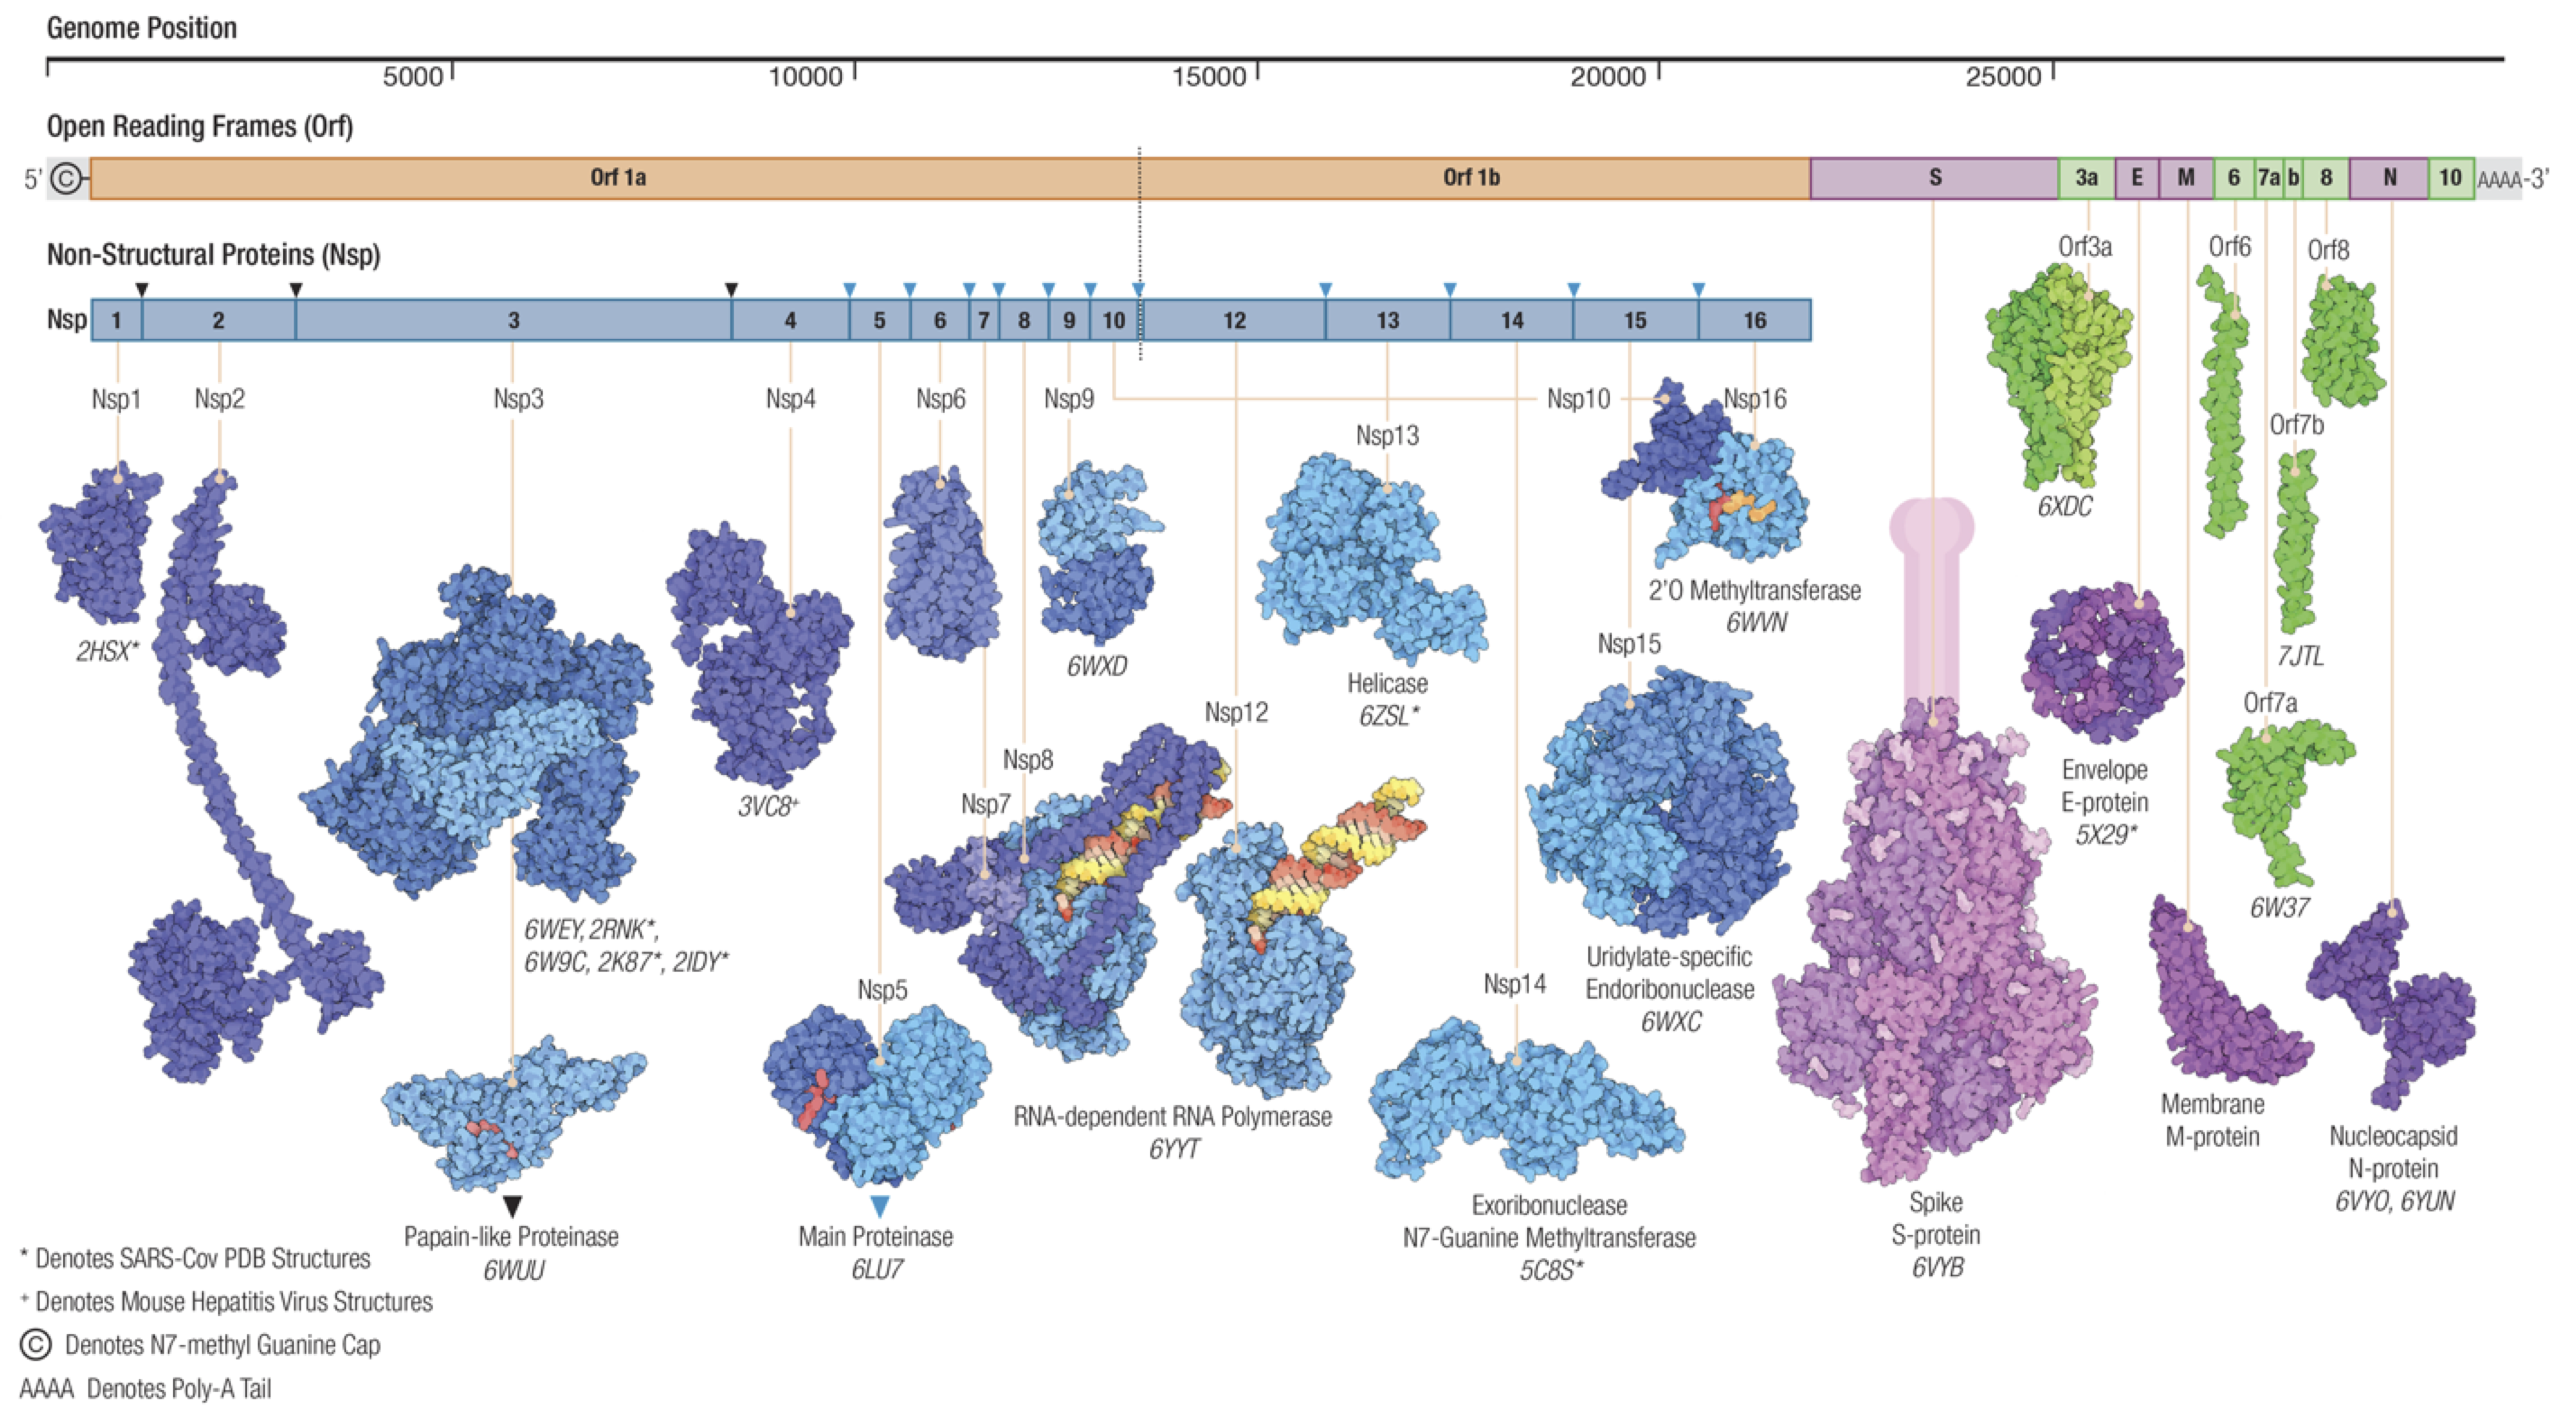
\includegraphics[width=\textwidth,keepaspectratio]{figures/covid_proteome.png}
	\caption{\textbf{Architecture of the SARS-CoV-2 genome and proteome.} Virion structural proteins spike (S), envelope (E), membrane (M) and nucleocapsid (N) are showed in purple. Current vaccines only elicit immunity to spike protein. Non-structural proteins are in shades of blue and open reading frame (Orf) proteins appear in green. Figure taken from \cite{covid3d}}
	\label{fig:covidprot}
\end{figure}

For many pathologies the major impediment to their study from an immunological repertoires perspective is the lack of these \textit{in-vitro}-determined antigen-specific TCRs \citep{tcrml}, but the scenario is somewhat better for COVID-19. In July 2020 Adaptive Biotechnologies and Microsoft publicly released data of MIRA assays including more than 160000 \covid-specific TCRs recognizing 269 different \covid{} epitopes \citep{immunecode}. These epitopes covered most of \covid{} proteins, shown in Fig. \ref{fig:covidprot}.

Several articles about \covid{} vaccines eliciting robust antibody responses against \covid{} spike (S) protein were published in high impact journals during early phase clinical trials \citep{pfizerab, janssenab, astrazenecaab} and later came the first preprints analyzing the immunogenicity of vaccines from a T cell and TCR repertoire perspective \citep{pfizertcr, janssen, astrazenecatcr}. However, these studies tend to analyze TCR repertoires in a very narrow manner, limiting their analysis to measure the frequencies of the \covid-specific TCRs found in a repertoire by an exact sequence match, and therefore probably underestimating the TCR response in COVID-19.

The present study aims to analyze in depth the published TCR repertoires of 19 COVID-19 convalescent individuals, 19 Ad26.COV2.S vaccine (developed by Janssen Pharmaceutica) recipient individuals and 5 placebo recipient individuals to fully characterize how viral and vaccine immunization alter the complex landscape of TCR repertoires in health and disease.



%%% TO-DO figure
